\documentclass[../main.tex]{subfiles}

\begin{document}

\section{Question 6}

Model using HDL a design that can be used to implement an arithmetic right shift. Your design has to be parametric and have N-bit input, where $N \geq 4$. It should also allow to shift up to 3 positions. Do \textbf{not} use the \texttt{<<<}, \texttt{>>>} operators.

Draw a schematic of your design. Assume a value for the parameter $N = 5$.

\subsection*{Solution}

The functionality can be implemented using an array of N-to-1 multiplexers. Denoting the input and output bit-vectors $d_i$ and $d_o$ respectively, and the 2-bit select line for $s$, the circuit schematic when $N = 5$ is shown in [Figure \ref{q6}].

\begin{figure}[h]
    \centering
    
\includegraphics[width=1.0\linewidth]{assets/q6.png}
    \caption{$N = 5$ right shifter implemented using an array of multiplexers.}
    \label{q6}
\end{figure}

The output from the testbench of the implemented circuit is shown below.

\begin{mintedterminal}{Q6 - Testbench Output}
[10] Starting simulation...
[010] Input=10101010 Control=0 Output=10101010
[020] Input=10101010 Control=1 Output=01010101
[030] Input=10101010 Control=2 Output=00101010
[040] Input=10101010 Control=3 Output=00010101
\end{mintedterminal}

\newpage

\section{Question 7}

Model using HDL a signed N-bit multiplier. The design has to be parametric with 2 inputs of N-bit, where $N > 3$. Your design should use half adders and/or full adders.

Draw the schematic of your design. Assume a value for the parameter $N = 5$.

\subsection*{Solution}

To implement signed multiplication the Baugh-Wooley multiplication algorithm is used. A Baugh-Wooley multiplier is implemented as a grid of "Baugh-Wooley cells". Two types of cells are used, white and gray [Figure \ref{fig:bw_cell}]. The complete circuit diagram is seen in [Figure \ref{q7}].

\begin{figure}[h]
    \centering
    \begin{subfigure}{.5\textwidth}
        \centering
        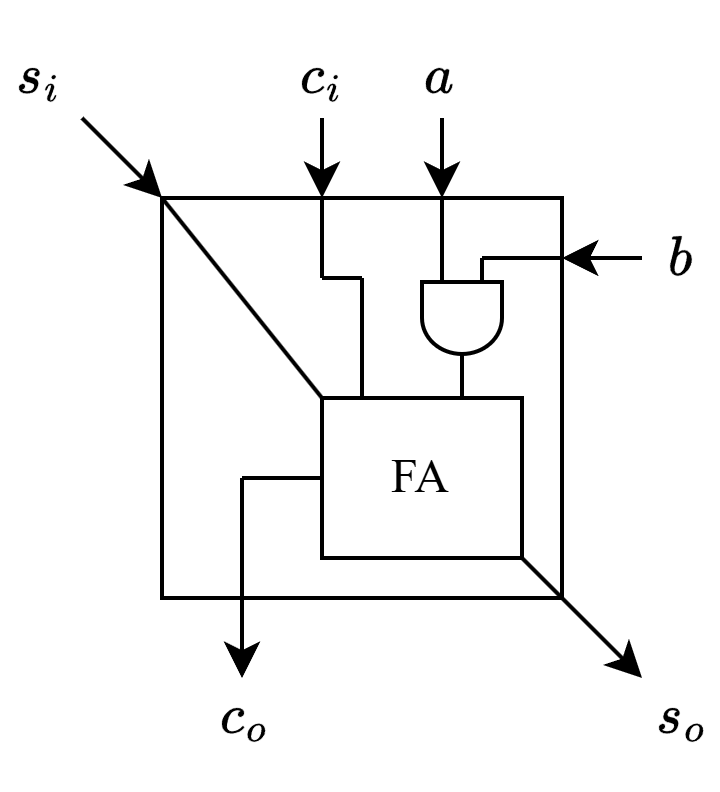
\includegraphics[width=0.8\linewidth]{assets/bw_white_cell.png}
        \vspace{-10pt}
        \caption{Baugh-Wooley multiplier white-cell.}
        \label{fig:bw_white_cell}
    \end{subfigure}%
    \begin{subfigure}{.5\textwidth}
        \centering
        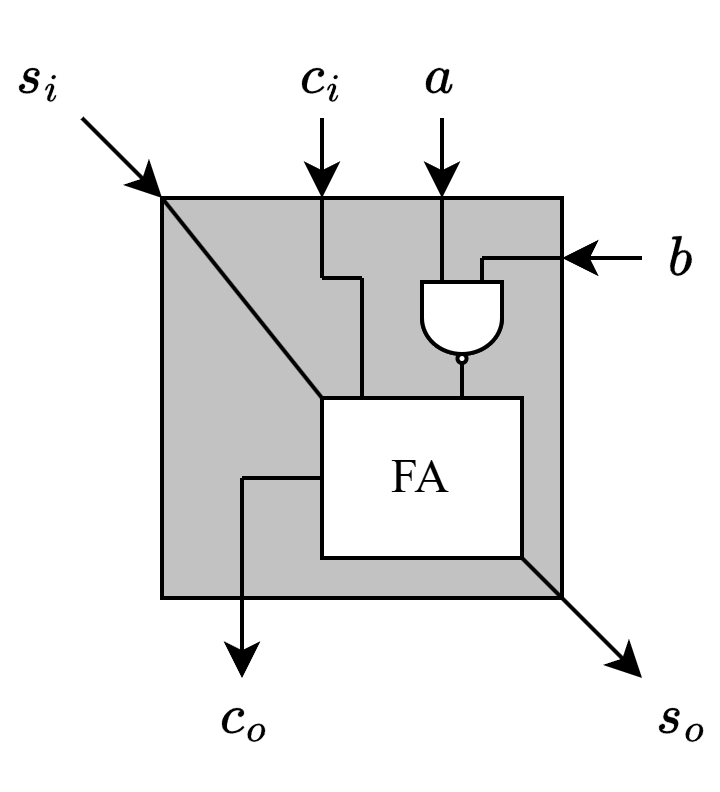
\includegraphics[width=0.8\linewidth]{assets/bw_gray_cell.png}
        \vspace{-10pt}
        \caption{Baugh-Wooley multiplier gray-cell.}
        \label{fig:bw_gray_cell}
    \end{subfigure}
    \vspace{-10pt}
    \caption{Baugh-Wooley multiplier basic cell construction.}
    \label{fig:bw_cell}
\end{figure}

\newpage

\begin{figure}[H]
    \centering
    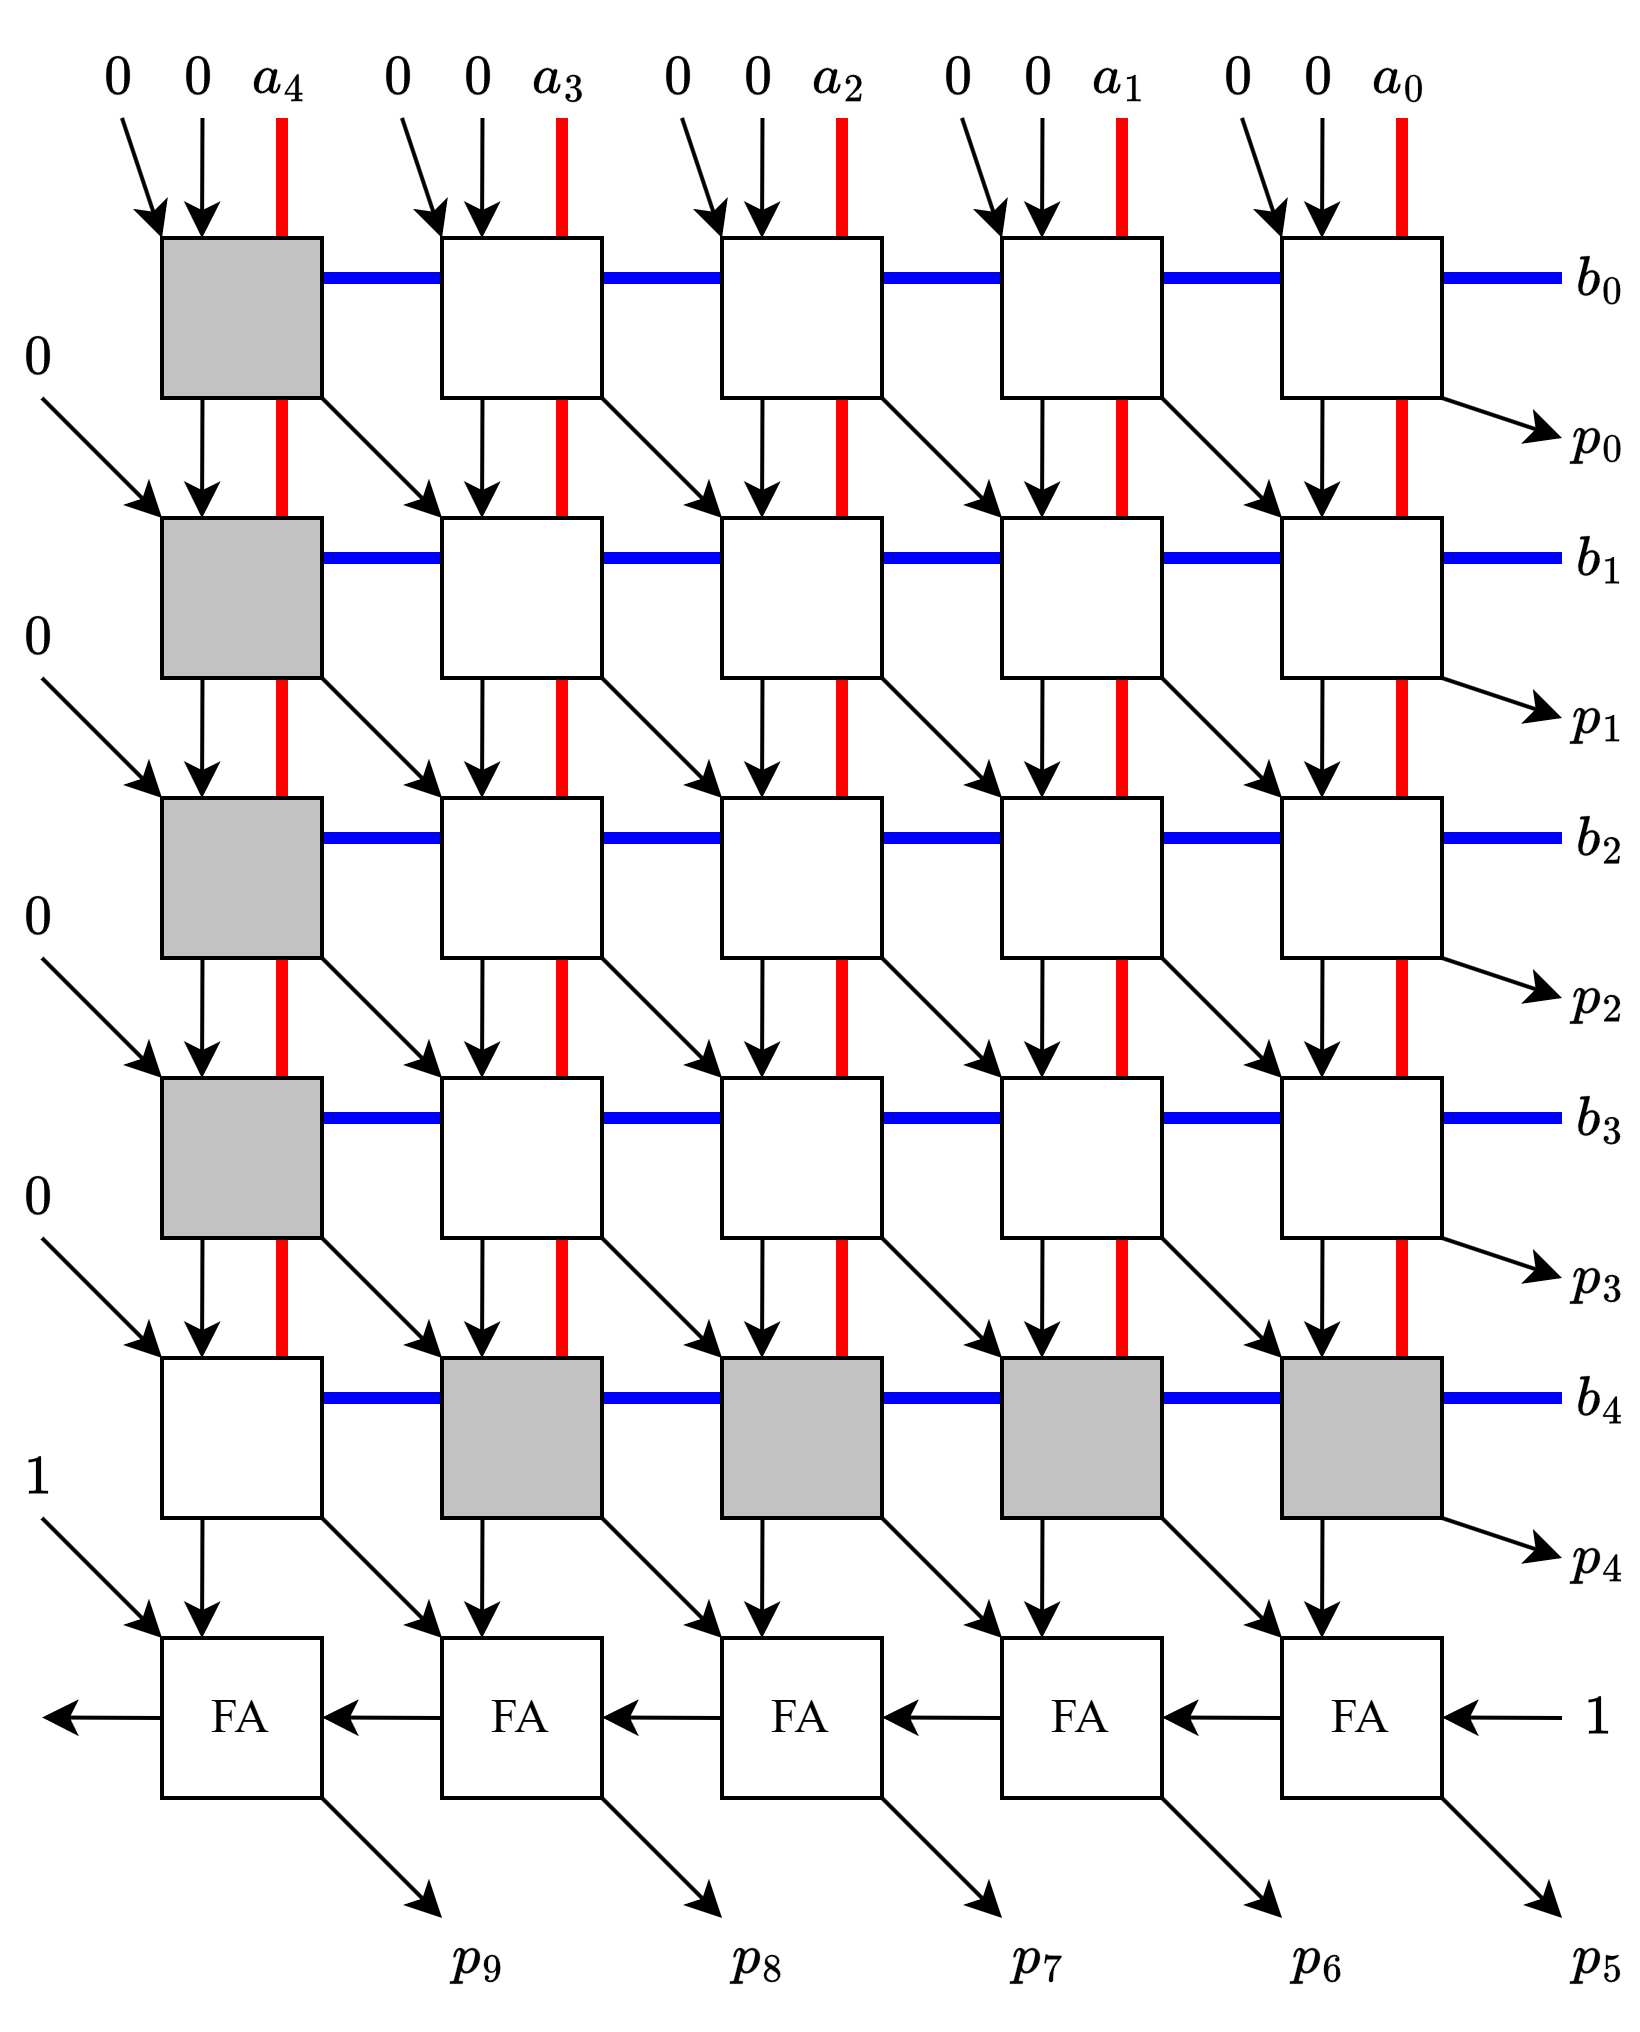
\includegraphics[width=1.0\linewidth]{assets/bw_5bit_multiplier.png}
    \caption{Block diagram of a $N = 5$ Baugh-Wooley multiplier implemented using basic Baugh-Wooley white- and gray-cells. Inputs are denoted $a$, $b$, and the product is denoted $p$.}
    \label{q7}
\end{figure}

\newpage

\section{Question 8}

Model using HDL a design that can multiply 6 N-bit numbers and add the results. The design should be parametric with parameter N. You must ensure that your design does not overflow or underflow and assign the correct bit width for all intermediate and output signals. The design should implement the following equation:

$$
    \text{out} = \sum_{k \in {0, 2, 4}} X_k \cdot X_{k + 1}
$$

Draw a schematic of your design. Assume a value for the $N = $ parameter.

\subsection*{Solution}

\end{document}
